\documentclass[10pt,journal,onecolumn]{IEEEtran}

\usepackage[utf8]{inputenc}
\usepackage[T1]{fontenc}
\usepackage{silence}\WarningsOff[latexfont]

\usepackage{amsmath}
\usepackage{amsfonts}
\usepackage{amssymb}

\usepackage{graphicx}
\graphicspath{images/}
\usepackage{cite}
\usepackage{url}
\usepackage{caption}
\usepackage{subcaption}
\usepackage{float}
\usepackage[ruled,vlined,linesnumbered]{algorithm2e}
\SetKwProg{Fn}{Event}{}{}
\SetKw{And}{and}
\usepackage[binary-units,per-mode=symbol]{siunitx}
\sisetup{list-final-separator = {, and },detect-weight=true, detect-family=true}
\usepackage{booktabs}
\usepackage{pifont}
\usepackage{microtype}
\usepackage{textcomp}
\usepackage[american]{babel}
\usepackage[capitalise]{cleveref}
\def\figname{\csname cref@figure@name\endcsname\xspace}
\def\tabname{\csname cref@table@name\endcsname\xspace}
\def\secname{\csname cref@section@name\endcsname\xspace}
\def\eqpname{\csname cref@equation@name@plural\endcsname\xspace}
\crefname{algorithm}{Listing}{Lists.}
\Crefname{algorithm}{Listing}{Listings}
\SetAlgorithmName{Listing}{Listing}{List of Listings}
\crefname{lstlisting}{listing}{listings}
\Crefname{lstlisting}{Listing}{Listings}
\usepackage{xspace}
\usepackage{hyphenat}
\usepackage[draft,inline,nomargin,index]{fixme}
\fxsetup{theme=color}
\usepackage{grffile}
\usepackage{xfrac}
\usepackage{multirow}
%\usepackage[para]{footmisc}
\usepackage[font={small}]{caption}
\usepackage{imakeidx}
\usepackage{longtable}
\usepackage[table]{xcolor}
\definecolor{lightgray}{gray}{0.9}
\let\oldlongtable\longtable

\let\endoldlongtable\endlongtable

\renewenvironment{longtable}{\rowcolors{2}{white}{lightgray}\oldlongtable} 
{\endoldlongtable}

\usepackage{tikz}
\usetikzlibrary{calc,shapes,arrows,fit,positioning}

\usepackage{listings}
\lstset{
   language=sh,
   columns=fixed,
   breaklines=true,
   breakatwhitespace=true,
   prebreak=\textbackslash,
   basicstyle=\ttfamily\small,
   showstringspaces=false,
   upquote=true,
   keywordstyle=\ttfamily\small
}

\usepackage{color}
\definecolor{gray}{rgb}{0.4,0.4,0.4}
\definecolor{darkblue}{rgb}{0.0,0.0,0.6}
\definecolor{cyan}{rgb}{0.0,0.6,0.6}


\lstdefinelanguage{XML}
{
  morestring=[b]",
  morestring=[s]{>}{<},
  morecomment=[s]{<?}{?>},
  stringstyle=\color{black},
  identifierstyle=\color{darkblue},
  keywordstyle=\color{cyan},
  morekeywords={xmlns,version,type}% list your attributes here
}

\definecolor{codegreen}{rgb}{0,0.6,0}
\definecolor{codegray}{rgb}{0.5,0.5,0.5}
\definecolor{codepurple}{rgb}{0.58,0,0.82}
\definecolor{backcolour}{rgb}{0.95,0.95,0.92}

\lstdefinestyle{shell}{
    backgroundcolor=\color{backcolour},
    breakatwhitespace=false,
    breaklines=true,
    captionpos=b,
    keepspaces=true,
    showspaces=false,
    showstringspaces=false,
    showtabs=false,
    tabsize=2
}

\lstdefinestyle{graphml}{
    backgroundcolor=\color{backcolour},
    breakatwhitespace=false,
    breaklines=true,
    captionpos=b,
    keepspaces=true,
    showspaces=false,
    showstringspaces=false,
    showtabs=false,
    tabsize=2
}

\lstMakeShortInline[language=bash]|

% fix cleveref and breqn
\makeatletter
\let\cref@old@eq@setnumberOld\eq@setnumber
\def\eq@setnumber{%
\cref@old@eq@setnumberOld%
\cref@constructprefix{equation}{\cref@result}%
\protected@xdef\cref@currentlabel{%
[equation][\arabic{equation}][\cref@result]\p@equation\eq@number}}
\makeatother

% reduce verbatim font size
\usepackage{etoolbox}
\makeatletter
\patchcmd{\@verbatim}
  %%%{\verbatim@font} %% blow up TexMaker formatting ???!!! 
  {\verbatim@font\small}
  {}{}
\makeatother

\RequirePackage{xstring}
\RequirePackage{xparse}
\RequirePackage[index=true]{acro}
\NewDocumentCommand\acrodef{mO{#1}mG{}}{\DeclareAcronym{#1}{short={#2}, long={#3}, #4}}
\NewDocumentCommand\acused{m}{\acuse{#1}}
\newcommand{\q}[1]{``#1''}

\acrodef{ADV}{advertisement}
\acrodef{AS}{Autonomous System}{short-plural=es}
\acrodef{BGP}{Border Gateway Protocol}
\acrodef{BIRD}{BGP Internet Routing Daemon}
\acrodef{DPC}{Destination Partial Centrality}
\acrodef{eBGP}{Exterior BGP}
\acrodef{ERP}{Exterior Routing Protocol}
\acrodef{IoF}{Internet on FIRE}
\acrodef{IP}{Internet Protocol}
\acrodef{MRAI}{Minimum Route Advertisement Interval}
\acrodef{NH}{Next Hop}
\acrodef{RFC}{Request For Comment} 
\acrodef{TCP}{Transmission Control Protocol}
\acrodef{FSM}{Finite State Machine}
\acrodef{DES}{Descrete Event Simulator}
\acrodef{RFD}{Route Flap Damping}
\acrodef{RNG}{Random Number Generator}
\acrodef{LID}{Link identifier}
\acrodef{RIB}{Routing Information Base}{short-plural=s}

\newcommand\useallac{
\acused{IP}
\acused{TCP}
\acused{RFC}
}

\useallac

\newcommand{\figwidthfour}{0.78}
\newcommand{\figwidth}{0.78}
\newcommand{\figvspace}{-1.5em}
\newcommand{\update}{\texttt{UPDATE}\xspace}
\newcommand{\nodeset}{\ensuremath{\mathcal{V}}\xspace}
\newcommand{\destinationset}{\ensuremath{\mathcal{C}}\xspace}
\newcommand{\edgeset}{\ensuremath{\mathcal{E}}\xspace}
\newcommand{\graph}{\ensuremath{\mathcal{G(\nodeset,\edgeset)}}\xspace}
\newcommand{\pathset}{\ensuremath{\mathcal{C}}\xspace}
\newcommand{\ascentg}{\ensuremath{\mathcal{G_{A}}\xspace}}
\newcommand{\ascentnodeset}{\ensuremath{\mathcal{V^{\ascentg}}}\xspace}
\newcommand{\ascentedgeset}{\ensuremath{\mathcal{E^{\ascentg}}}\xspace}
\newcommand{\ascentgraph}{\ensuremath{\mathcal{\ascentg(\ascentnodeset,\ascentedgeset)}}\xspace}
\newcommand{\dpc}{\ensuremath{\Delta}\xspace}
\newcommand{\tr}{\ensuremath{T_{R}}\xspace}

\newcommand{\tierg}{\ensuremath{\mathcal{G_{T}}\xspace}}
\newcommand{\tiernodeset}{\ensuremath{\mathcal{V^{\tierg}}}\xspace}
\newcommand{\tieredgeset}{\ensuremath{\mathcal{E^{\tierg}}}\xspace}
\newcommand{\tiergraph}{\ensuremath{\mathcal{\tierg(\tiernodeset,\tieredgeset)}}\xspace}
\newcommand{\descentg}{\ensuremath{\mathcal{G_{D}}\xspace}}
\newcommand{\descentnodeset}{\ensuremath{\mathcal{V^{\descentg}}}\xspace}
\newcommand{\descentedgeset}{\ensuremath{\mathcal{E^{\descentg}}}\xspace}
\newcommand{\descentgraph}{\ensuremath{\mathcal{\descentg(\descentnodeset,\descentedgeset)}}\xspace}

\IEEEoverridecommandlockouts
\makeindex[columns=3, title=Alphabetical Index, intoc]

\begin{document}

\title{User Manual BGP simulator}
\author{
	\IEEEauthorblockN{Mattia Milani}\\
    \IEEEauthorblockA{Dept. of Information Engineering and Computer Science, University of Trento, Italy}
    \texttt{mattia.milani@studenti.unitn.it}
}


\maketitle

\clearpage

\tableofcontents

\clearpage

\section{Guide environment}
\label{sec:guide_environment}

This guide has been tested on a clean installation of ubuntu 18.04
with python 3.6.9

\section{Experiments general chain}
\label{sec:general_chain}

This environment is composed by different components, thats executed one after
the other will produce the output expected.

\begin{figure}[h]
	\begin{center}
		\begin{tikzpicture}[scale=0.2]
			\tikzstyle{every node}+=[inner sep=0pt]
			\draw [black] (0,0) rectangle (10,5);
			\draw [black] (20,0) rectangle (30,5);
			\draw [black] (40,0) rectangle (50,5);
			\draw [thick, ->] (10,2.5) -- (20,2.5);
			\draw [thick, ->] (30,2.5) -- (40,2.5);
			\node [DES] at (5,2.5) {DES};
			\node [Analyzer] at (25,2.5) {Analyzer};
			\node [Plotter] at (45,2.5) {Plotter};
		\end{tikzpicture}
	\end{center}
	\caption{General environment chain}
	\label{fig:general_chain}
\end{figure}

\Cref{fig:general_chain} shows how in general an experiment is conducted.
The first step is the \ac{DES} that takes in input some configuration files
and runs each step of the simulation.
The network simulated evolves producting some output files in \textit{CSV} format
that would be the input for the next step.
The second part of this environment is take by the analyzer, it's the main
interpreter of the \ac{DES} output, it takes as input the CSVs files produced
by the first step. The output of the analyzer is another set of CSVs that are
easily plottable or that represent in a more clean way some aspectes of the simulations.
The analyzer can take as input multiple \ac{DES} execution and produce mean
results.
The analyzer is a necessary step to merge multiple experiments, it is also
necessary because from a single \ac{DES} execution is possible to study
a lot of different aspects (Time convergence, number of messages, a single node
evolution, etc.) and is not always necessary to study all this aspects.
The last part of an experiment is the plotter.
This part take as input CSV files created by the analyzer and simply plot what
is in them.

Each component is necessary to reach the goal of an experiment.

\section{How to install}
\label{sec:installation}

This section contains an explanation on how to install in the correct
way the software required by the environment.

In the main src folder of the project is present a bash file that will install
everything you need, just use the following commands:

\lstset{style=shell}
\begin{lstlisting}[language=bash]
	cd src/
	./install.sh
\end{lstlisting}

This code will execute the default installation process, is possible to modify the default
values using the install script arguments.

use: 
\begin{lstlisting}[language=bash]
	./install.sh -h
\end{lstlisting}
to see the argument description.

The installation script will automatically install the following packets:
\begin{itemize}
		\item python-virtualenv, permits the use of python virtual environment,
			used to create the environment where all the python libraries and packages
			will be installed
		\item parallel, permits the execution of parallel commands/scripts and
			a lot more things, used to run multiple experiments in parallel
		\item graphviz, used to produce some graphs after the analysis part.
		\item gcc, required by the pygraphviz package
		\item python3-dev, required by some packages installed
\end{itemize}
The installation script will also create a virtual env for the python packages
required and then install all the python packages necessary.
use:
\begin{lstlisting}[language=bash]
	./install.sh -n <env-name>
\end{lstlisting}
to redefine the virtual environment default name (env).
The second argument that is possible to pass to the installation script is
the position of the python interpreter.
The default is the output of the command |which python3|, is possible to modify
it with:
\begin{lstlisting}[language=bash]
	./install.sh -p <path-to-python-interpreter>
\end{lstlisting}

The suggested python interpreter is the version 3.6.9, the one that has been tested.

The list of python packages that will be installed is contained in the file
|requirements.txt|.

At the end of the installation will be possible to use the virtual environment
just created, use the following command to activate the virtual environment:
\begin{lstlisting}[language=bash]
	source /<env-name>/bin/activate
\end{lstlisting}
To deactivate an environment use the command:
\begin{lstlisting}[language=bash]
	deactivate
\end{lstlisting}

For compatibilities problems with libraries versions and python versions
please contact me.

\section{Experiments configuration files}
\label{sec:exp_conf}

To execute an experiment are necessary some configuration files that define how
the environment is setted and generated.
For example is possible to define which nodes are in the network and the connections
between one another, then is possible to configure the single node properties.
Another configuration file permits to configure the general properties of the
experiment, for example: the signal that the source nodes should share, the 
maximum experiment duration ecc.

All this parameters are divided in two files that are here presented.
The approach to those files in this document is the following:
in the \Cref{subsec:graph_file,subsec:json_file} all the configuration properties
are presented.
in the following sections all these properties are displayed in an 
increasingly complete way until you see each of them.
Some of them are not compatible one another.

\subsection{Graph file}
\label{subsec:graph_file}

The graph file is the one that describes the network. though it is possible
to define the nodes of the experiment and te relation between one another.
The format chosen for this file is the graphml format, that gives enough liberty
to define all the topological properties of the network.

The common structure of the graphml file is the following:
% TODO color the main arguments
\begin{lstlisting}[language=bash]
	<?xml version='1.0' encoding='utf-8'?>
	<graphml xmlns="http://graphml.graphdrawing.org/xmlns" xmlns:xsi="http://www.w3.org/2001/XMLSchema-instance" xsi:schemaLocation="http://graphml.graphdr    awing.org/xmlns http://graphml.graphdrawing.org/xmlns/1.0/graphml.xsd">
	  <attributes/>
	  <graph edgedefault="directed">
		< nodes section />
	    <node id="0">
			< node attributes />
	    </node>
		< edges section />
	    <edge source="0" target="1">
			< edge attributes />
	    </edge>
	  </graph>
	</graphml> 
\end{lstlisting}

an example of simple graph is given by the following graphml code:
\lstset{style=graphml}
\renewcommand{\lstlistingname}{Conf file}
\begin{lstlisting}[language=bash, caption=first graph file, label=graph:first_graphml]
	<?xml version='1.0' encoding='utf-8'?>
	<graphml xmlns="http://graphml.graphdrawing.org/xmlns" xmlns:xsi="http://www.w3.org/2001/XMLSchema-instance" xsi:schemaLocation="http://graphml.graphdr    awing.org/xmlns http://graphml.graphdrawing.org/xmlns/1.0/graphml.xsd">
	  <key attr.name="destinations" attr.type="string" for="node" id="d0" />
	  <key attr.name="delay" attr.type="string" for="edge" id="d1" />
	  <graph edgedefault="directed">
	    <node id="0">
	        <data key="d0">10.0.0.0/24,10.0.1.0/24</data>
	    </node>
	    <node id="1">
	        <data key="d0">10.0.2.0/24,10.0.3.0/24</data>
	    </node>
	    <node id="2">
	    </node>
	    <node id="3">
	    </node>
	    <edge source="0" target="1">
	        <data key="d1">{"distribution": "unif", "min": 1, "max": 5, "int": 0.01}</data>
	    </edge>
	    <edge source="0" target="3">
	    </edge>
	    <edge source="1" target="0">
	    </edge>
	    <edge source="1" target="2">
	    </edge>
	    <edge source="2" target="1">
	    </edge>
	    <edge source="1" target="3">
	    </edge>
	    <edge source="3" target="1">
	    </edge>
	  </graph>
	</graphml>
\end{lstlisting}

that represent the following graph:
\begin{figure}[h]
	\begin{center}
		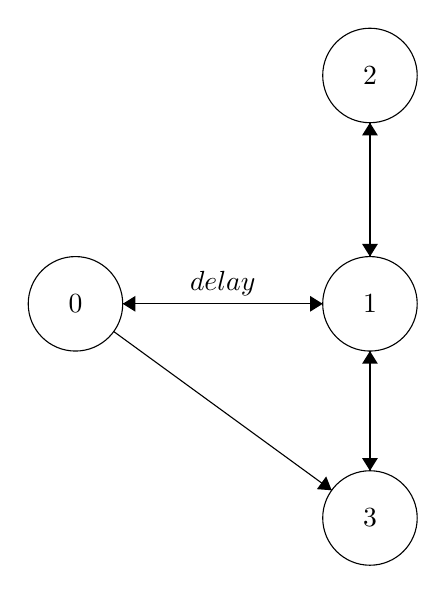
\begin{tikzpicture}[scale=0.2]
			\tikzstyle{every node}+=[inner sep=0pt]
			\draw [black] (24.9,-18.3) circle (3);
			\draw (24.9,-18.3) node {$0$};
			\draw [black] (43.6,-18.3) circle (3);
			\draw (43.6,-18.3) node {$1$};
			\draw [black] (43.6,-3.8) circle (3);
			\draw (43.6,-3.8) node {$2$};
			\draw [black] (43.6,-31.9) circle (3);
			\draw (43.6,-31.9) node {$3$};
			\draw [black] (27.9,-18.3) -- (40.6,-18.3);
			\fill [black] (40.6,-18.3) -- (39.8,-17.8) -- (39.8,-18.8);
			\draw (34.25,-17.8) node [above] {$delay$};
			\draw [black] (27.33,-20.06) -- (41.17,-30.14);
			\fill [black] (41.17,-30.14) -- (40.82,-29.26) -- (40.23,-30.07);
			\draw [black] (40.6,-18.3) -- (27.9,-18.3);
			\fill [black] (27.9,-18.3) -- (28.7,-18.8) -- (28.7,-17.8);
			\draw [black] (43.6,-15.3) -- (43.6,-6.8);
			\fill [black] (43.6,-6.8) -- (43.1,-7.6) -- (44.1,-7.6);
			\draw [black] (43.6,-6.8) -- (43.6,-15.3);
			\fill [black] (43.6,-15.3) -- (44.1,-14.5) -- (43.1,-14.5);
			\draw [black] (43.6,-21.3) -- (43.6,-28.9);
			\fill [black] (43.6,-28.9) -- (44.1,-28.1) -- (43.1,-28.1);
			\draw [black] (43.6,-28.9) -- (43.6,-21.3);
			\fill [black] (43.6,-21.3) -- (43.1,-22.1) -- (44.1,-22.1);
		\end{tikzpicture}
	\end{center}
	\caption{Graphml graphical representation}
	\label{fig:first_graph_representation}
\end{figure}

As we can notice in graphml file \ref{graph:first_graphml} nodes \num{0} and \num{1} uses the attribute $d0$ that
defines a property of them (all the properties are listed below).
In the edges section is alto noticable that a delay attribute is used between
node \num{0} and \num{1}.

The graph must be directed

All the accepted properties for nodes are listed below:
\begin{itemize}
		\item destinations:  This attribute represent the networks that a node will share 
			during the experiment, it is possible to intrudce multiple networs 
			separated by a |,|;
		\item MRAI\_affects\_withdraws: This attribute defines if the node does not 
			applys the suggested RFC \fixme{insert citation} where is defined that
			MRAI does not affect withdraws, insert a value higher than \num{0} to
			activate this function;
		\item RFD: Route flap damping, this attribute defines the parameters
			that the node will use to configure its own route flap dampening
			procedure;
		\item centrality: Float value that defines the centrality of the node;
		\item type: String attribute that defines the type of the node.
\end{itemize}
The type of a node could be one from the following:
\begin{itemize}
		\item T: tier one node;
		\item M: Nodes that act as proveders for clients;
		\item CP: Client providers nodes;
		\item C: Client nodes.
\end{itemize}
The \ac{RFD} configuration parameters are described in \Cref{subsec:RFD}.

All the accepted properties for edges are listed below:
\begin{itemize}
		\item delay: {distribution} is possible to introduce a delay distribution 
			for a single edge, the distribution has to respect what said in the 
			distribution section of the readme. This parameter will override the 
			json delay parameter for the edge;
		\item policy: is possible to define a policy function for every single edge, 
			policy functions are applyied like explanied in \fixme{insert citation} 
			see the section policy function for more deep explanations, default: pass everything;
		\item mrai: is possible to define an \ac{MRAI} value for each edge, this 
			float value would override the default one of
			30.0 seconds, like defined in \fixme{citation rfc 4271}.
\end{itemize}

Refers respecively to \Cref{subsec:distribution,subsec:policies} for an explanation
about distributions that can be used and how policies can be setted.

Examples of complex graphs are contained in the |graphs| folder and some of them
are exmplained in the next chapters.

\subsection{Json file}
\label{subsec:json_file}

To define environment variables is possible to use a json file that must be 
passed to the DES. 
Examples of configuration file is available in: |/src/json/|

The parameters that can be defined inside the json file are:
\begin{itemize}
    \item seed: this variable represents the seed that will be passed to 
		the \ac{RNG} at the environment initialization
    \item duration: Duration of each run in seconds
    \item graph: Graphml file that will be used for all the runs
    \item output: Represent the output file of each run. is possible to use 
		other variables inside the string, for example |{date-time}| will be 
		substituted by the actual dateTime of the experiment (up to ms) or 
		is possible to use other variables like |{seed}| or |{withdraw_dist.min}|
		to introduce more levels of details to recognize the output csv 
		file among many of a multi run script
    \item verbose: |[True/False]| variable, if true the experiment will 
		print the evolution on standard output
	\item signaling: |[True/False]| variable, if true the experiment will use 
		the signaling sequence defined in |signaling_sequence|, nodes that contains
		a destination will respect this sequence using the withdraw and reannouncement
		distribution.
		If false the evolution will be based on the \ac{RNG} and limited only
		by the |duration|.
	\item signaling\_sequence: |"AWAW..."| string variable composed by a 
		sequence of announcements and withdraws, this will be the execution sequence
		for nodes that share a destination.
	\item implicit\_withdraw: |[True/False]| variable, if True nodes will 
		use the implicit withdraw schema (a new path for a neighbour is the sum
		of a withdraw of the previous path and the announcement of the new 
		best path) if false nodes that change best path will send a withdraw 
		followed by an announcement.
    \item withdraw: |[True/False]| variable, if true a node that previusly 
		shared a network it will produce a withdraw of the network after a delay 
		time described by |withdraw_dist|
    \item reannouncement: |[True/False]| variable, if true a node that previusly 
		withdrawed a route will schedule a reannouncement of the route 
		using the distribution described in |reannouncement_dist|
    \item withdraw\_dist: Variable that describe a withdraw distribution, 
		for a distributions explanation please see \Cref{subsec:distribution}
    \item reannouncement\_dist: Like the withdraw distribution but for reannouncements
    \item datarate: |{distribution}| Time required to start the actual 
		transmission of a message after the scheduling
    \item processing: |{distribution}| Processing time of any information, 
		for example can be used after the reception of a packet to 
		simulate the processing of it
    \item delay: |{distrbution}| Network delay for the packets on links.
\end{itemize}

All parameters can be array of parameters, so is possible to run different 
combinations of them.
An array of parameters could be the following:
|seed: [0, 1, 2, 3]| -> this defines multiple seeds that can be used

\begin{lstlisting}[language=bash]
	"withdraw_dist": [{"distribution": "unif", "min": 5, "max": 10, "int": 0.1}, 
					  {"distribution": "unif", "min": 8, "max": 10, "int": 0.1}, 
					  {"distribution": "unif", "min": 2, "max": 3, "int": 0.1}]
\end{lstlisting}

An example of compleate json file:
\renewcommand{\lstlistingname}{Conf file}
\begin{lstlisting}[language=bash, caption=Example of json file, label=json:line_example]
	{                                                                               
	    "line" : {                                                                  
	        // seed(s) to initialize PRNGs                                          
	        "seed" : [0, 1, 2, 3, 4, 5, 6, 7, 8, 9],                                
	        // duration of each simulation in seconds                               
	        "duration" : 60000,                                                     
	        // Graph file to simulate                                               
	        "graph": "graphs/tests/line.graphml",    
	        // log file name using configuration parameters, use {seed} or {date-time}
	        "output" : "results/line/line_{seed}.csv",
	        // Verbose value                                                        
	        "verbose": "True",                                                      
	        // Signaling flag                                                       
	        "signaling": "True",                                                    
	        // Signaling sequence, ignored if signaling false                       
	        "signaling_sequence": "AWAWAWA",                                        
	        // Implicit withdraw of routes                                          
	        "implicit_withdraw": "True",                                            
	        // Withdraw signaling                                                   
	        "withdraw": "True",                                                     
	        // Reannouncement of a destination after a withdraw                     
	        "reannouncement": "False",                                              
	        // Withdraw interval distribution from the announcement                 
	        "withdraw_dist": {"distribution": "const", "mean": 300},                
	        // announcement interval distribution from the withdraw                 
	        "reannouncement_dist": {"distribution": "const", "mean": 300},          
	        // Transmission time required to start the actual message transmission  
	        "datarate": {"distribution": "exp", "lambda" : 100},                    
	        // Processing time distribution                                         
	        "processing": {"distribution": "const", "mean": 0.00001},               
	        // Network delay distribution                                           
	        "delay": {"distribution": "unif", "min": 0.012, "max": 3, "int": 0.001} 
	    }                                                                           
	}   
\end{lstlisting}
In Conf file \ref{json:line_example} is possible to see that the the only vector
parameter is the |seed|.
The results of the simulations will be saved using the path given in the |output|
command, plus substituting the seed used in the csv file name.
the results folder is mandatory, it must already exists, while all the other 
folders will be created on the fly by the software.
From the signaling parameter is also possible to notice that this is a signaling
experiment, this means that the nodes that contains at least one destination will
only transmit messages respecting the given sequence.

\subsection{Distributions}
\label{subsec:distribution}

Up to now the possible distributions that can be itroduced in the environment are the following:

\begin{itemize}
    \item Uniform: a uniform distribution will have like name unif and 3 parameters 
		min that represent the minimum value that can be choose max the maximum 
		value int that represent the precision used for all the values between 
		min and max, all parameters can be float values
    \item Exponential: an exponential distribution have like name exp and it has 
		a parameter lambda, like for the uniform distribution the parameter can 
		be a float value
    \item Constant: a constant distribution have like name: const and it has one 
		parameter named mean
\end{itemize}

All the values of the distributions are intended in seconds.

An example of distribution: |{"distribution": "const", "mean" : 0.00001}|

Distributions used in the graph to override the standard delay:
\begin{lstlisting}[language=bash]
 <edge source="0" target="1">
     <data key="d1">{"distribution": "unif", "min": 1, "max": 5, "int": 0.01}</data>
 </edge>
\end{lstlisting}

\subsection{Policies}
\label{subsec:policies}

A policy function is applied like exporter filter. If the value returned by the 
function is not infinite the route will be sent with the value returned by f

policy functions are formally explained in \fixme{insert citation} Sec IV-c

An example of policy function could be this: |<1, inf, inf>|

This policy can simulate the peer behaviour of a node. It can send only routes 
that have a policy level of 0 and will substitute to the route the policy level 
with 1 before the actual transmission.

In the graphml file is mandatory to not use |<| and |>| simbols, so a function can 
be easily defined with:

|2, 2, 2|

Rotues that are originated by nodes will receive a policy level of \num{0} automatically.

Policy function used in a graphml file on an edge to define the relationship
between nodes:
\begin{lstlisting}[language=bash]
  <edge source="5" target="2">
      <data key="d2">0, inf, inf</data>
  </edge>
  <edge source="2" target="5">
      <data key="d2">2, 2, 2</data>
  </edge>
\end{lstlisting}

\subsection{RFD}
\label{subsec:RFD}

Refers to \fixme{insert citation} for a deep explanation about \ac{RFD} and its
parameters.

The \ac{RFD} system of a node is composed by multiple parameters:
\begin{itemize}
		\item Withdraw penalty: penalty applied to the figure of merit in case 
			of a withdraw reception
		\item Re-announcement penalty: penalty applied to the figure of merit
			in case of a re-announcement
		\item Attribute change penalty: penalty applied to the figure of merit
			in case of an attribute change.
		\item Suppression threshold (cut): threshold after which a route is 
			suppressed
		\item Reuse threshold: threshold after which a route is usable again
		\item T-hold timer: maximum time that a route could be suppressed
		\item Decay ok: decay time used if the route is reachable, half-life time
		\item Decay ng: decay time used if the route is not reachable, half-life time
		\item Decay memory limit ok: max time for which the memory of the figure
			of merit is kept if the route is reachable
		\item Decay memory limit ng: max time for which the memory of the figure
			of merit is kept if the route is not reachable;
		\item delta-t: time granularity in seconds used to perform all decay computations.
\end{itemize}	

An \ac{RFD} configuration is composed by all this attributes one after the other
in the same line separated by a "|,|".
The |rfd_setter.py| can be used to set an \ac{RFD} configuration for each node in 
a graph, is described in \Cref{sec:graph_generator}.

An example of \ac{RFD} configuration is the following:
\begin{lstlisting}[language=bash]
	1.0, 0.0, 0.5, 2.0, 0.75, 3600, 900, 900, 3600, 3600, 5
\end{lstlisting}

An example of \ac{RFD} configuration in a graphml file:
\begin{lstlisting}[language=bash]
	<node id="0">
	  <data key="d0">1.0, 0.0, 0.5, 2.0, 0.75, 3600, 900, 900, 3600, 3600, 5</data>
	</node> 
\end{lstlisting}

\section{Discrete event simulations}
\label{sec:des}

The simulator is the main component of the project, it permits to execute
experiments with different environments with the predefined topology.

\begin{figure}[h]
	\begin{center}
		\begin{tikzpicture}[scale=0.2]
			\tikzstyle{every node}+=[inner sep=0pt]
			\draw [black] (0,0) circle (4);
			\draw [black] (14,0) circle (4);
			\draw [black] (24,-2.5) rectangle (38,2.5);
			\draw [black] (48,0) circle (4); 
			\draw [thick, ->] (4,0) -- (10,0);
			\draw [thick, ->] (18,0) -- (24,0);
			\draw [thick, ->] (38,0) -- (44,0);
			\node [Graphml] at (0,0) {Graphml};
			\node [Json] at (14,0) {json};
			\node [DES] at (31,0) {DES};
			\node [Output] at (48,0) {Output};
		\end{tikzpicture}
	\end{center}
	\caption{Discrete event simulator structure}
	\label{fig:des_structure}
\end{figure}

The \ac{DES} receives as input a json file with all the environment parameters
that will be used during the experiment.
The output of the experiment could be divided in two category:
\begin{itemize}
	\item Standard output: The simulator will print messages on the standard
		output if the verbose option of the configuration file is active
	\item CSV files: the simulator will save events on the csv file
		configured as output in the json file.
\end{itemize}

The CSV file is mandatory, so the simulator will at least print the events 
sequence on that file.

The python file that act as entry point for the simulator is |src/fsm.py|.

\subsection{Simulator arguments}
\label{subsec:des_param}

The command:

\begin{lstlisting}[language=bash]
	python3 fsm.py --help
\end{lstlisting}

If an error message of a missing library is displayed, rembember to source the 
environment using |source env/bin/activate| before using the software of 
the repository.
Inside the folder |src/json/examples| there are some json examples that I will use
now to explain the different arguments that the simulator requires.

We will look to the file |line.json|.
If you open the file you can notice that the file is composed by two json parts.
The first one has as name |simulation| the second one |line|.

\begin{lstlisting}[language=bash]
{
	"simulation" : {
		....
	},
	"line" : {
		....
	}
}
\end{lstlisting}

Now we will take a look to the argument |-l| or |--list|, this argument has
the function to list all the available simulations in the standard output.

Try to run:
\begin{lstlisting}[language=bash]
	python3 fsm.py -c json/examples/line.json -l
\end{lstlisting}

The |-c| attribute is mandatory and defines which json file should be used by the
simulator.

The output should be:
\begin{lstlisting}[language=bash]
./fsm.py -c json/tests/line.json -s simulation -r 0
./fsm.py -c json/tests/line.json -s simulation -r 1	
\end{lstlisting}

This command has not executed the simulation, but it gives us some information
about the environment.
As default, if not specified the simulator will use the environment named 
simulation.
So it has looked into the json file, it has found the |simulation| environment
and it has gives us the list of different runs that we can execute with that
environment.

As you have probably imanginated up to now the parameter |-s| can be used
to pass the environment that we want to use in the simulation.
Infact if we use the following command we will obtain the same output as before:

\begin{lstlisting}[language=bash]
	python3 fsm.py -c json/examples/line.json -s simulation -l
\end{lstlisting}

The simulator has retrieved two lines, the first one endup with |-r 0| and the
second one with |-r 1|.
Thats because in the |simulation| environment we have a single vector of two 
elements, that is the seed.
\begin{lstlisting}[language=bash]
{
	"simulation" : {
		"seed" : [0, 1],
		....
	},
	"line" : {
		....
	}
}
\end{lstlisting}
The simulator recognize that we can run two different runs with the |simulation|
environment and it gives us the option to decide wich one using the |-r| argument.
It will assign a number to each combination of parameters that we have in
the environment.

With one single vector is easy to know which one correspond to which run number.
but with a more complex one?
For this purpose comes in help the |-L| or |--LIST| argument.

The following command will gives us a lot of information about the parameters
of the environment that we are using and the combination of values.

\begin{lstlisting}[language=bash]
	python3 fsm.py -c json/examples/line.json -s simulation -L
\end{lstlisting}

The ouput is:
\begin{lstlisting}[language=bash]
./fsm.py -c json/tests/line.json -s simulation -r 0: seed: 0
./fsm.py -c json/tests/line.json -s simulation -r 1: seed: 1
\end{lstlisting}

Now we know that to the index of run 0 correspond the seed 0 and to the 
index 1 correspond the seed 1.

The last argument is a flag |-g| you will see the result of this flag in the next
chapter where is explained the first experiment.
This argument will disable the rendering of the graph at the end of the simulation
if instad you leave this function untouched in the output folder will be
present also a graph rendered using networkx in the output folder.

Now lets take a look to a more complex environment.
Instead of the simulation environment try the line one with the |-l| and |-L|
parameters you will see that with more parameters vectors you will have a lot 
more runs that are possible.
The number of runs is always equal to the number of possible combination of 
all the parameters.

\begin{lstlisting}[language=bash]
	python3 fsm.py -c json/examples/line.json -s line -l
	python3 fsm.py -c json/examples/line.json -s line -L
\end{lstlisting}

\subsection{First experiment}
\label{subsec:first_exp}

For the first experiment we will use the |src/json/examples/line.json| with the
|simulation| environment lets take a look at it.

\begin{lstlisting}[language=json]
	"simulation" : {
		// seed(s) to initialize RNGs
		"seed" : [0, 1],
		// duration of each simulation in seconds
		"duration" : 600,
		// Graph file to simulate
		"graph": "graphs/general_tests/simple_line.graphml",
		// log file name using configuration parameters, use {seed} or {date-time}
		"output" : "results/tests/line/line_{seed}.csv",
		// Verbose value
		"verbose": "True",
		// Signaling flag
		"signaling": "False",
		// Signaling sequence, ignored if signaling false
		"signaling_sequence": "",
		// Implicit withdraw of routes
		"implicit_withdraw": "True",
		// Withdraw signaling
		"withdraw": "True",
		// Reannouncement of a destination after a withdraw
		"reannouncement": "True",
		// Withdraw interval distribution from the announcement
		"withdraw_dist": {"distribution": "const", "mean": 300},
		// announcement interval distribution from the withdraw
		"reannouncement_dist": {"distribution": "const", "mean": 300},
		// Transmission time required to start the actual message transmission
		"datarate": {"distribution": "exp", "lambda" : 100},
		// Processing time distribution
		"processing": {"distribution": "const", "mean": 0.00001},
		// Network delay distribution
		"delay": {"distribution": "unif", "min": 0.012, "max": 3, "int": 0.001}
	}
\end{lstlisting}

The graph that will be used could be represente by \Cref{fig:simple_line}
\begin{figure}[h]
	\begin{center}
		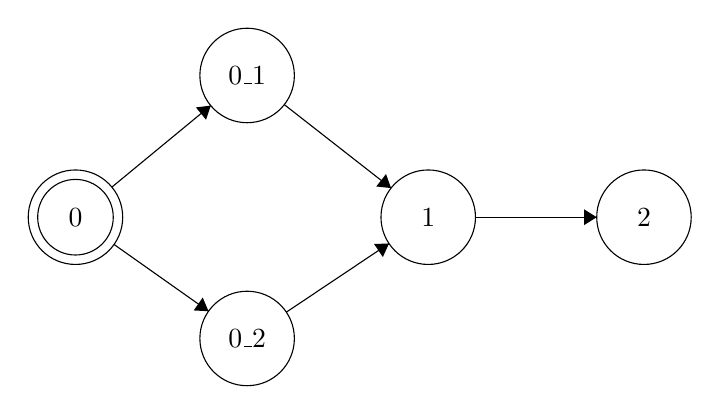
\begin{tikzpicture}[scale=0.2]
			\tikzstyle{every node}+=[inner sep=0pt]
			\draw [black] (10.7,-26.5) circle (3);
			\draw (10.7,-26.5) node {$0$};
			\draw [black] (10.7,-26.5) circle (2.4);
			\draw [black] (21.6,-17.5) circle (3);
			\draw (21.6,-17.5) node {$0\_1$};
			\draw [black] (21.6,-34.2) circle (3);
			\draw (21.6,-34.2) node {$0\_2$};
			\draw [black] (33.1,-26.5) circle (3);
			\draw (33.1,-26.5) node {$1$};
			\draw [black] (46.8,-26.5) circle (3);
			\draw (46.8,-26.5) node {$2$};
			\draw [black] (13.01,-24.59) -- (19.29,-19.41);
			\fill [black] (19.29,-19.41) -- (18.35,-19.53) -- (18.99,-20.31);
			\draw [black] (13.15,-28.23) -- (19.15,-32.47);
			\fill [black] (19.15,-32.47) -- (18.78,-31.6) -- (18.21,-32.42);
			\draw [black] (23.96,-19.35) -- (30.74,-24.65);
			\fill [black] (30.74,-24.65) -- (30.42,-23.76) -- (29.8,-24.55);
			\draw [black] (24.09,-32.53) -- (30.61,-28.17);
			\fill [black] (30.61,-28.17) -- (29.66,-28.2) -- (30.22,-29.03);
			\draw [black] (36.1,-26.5) -- (43.8,-26.5);
			\fill [black] (43.8,-26.5) -- (43,-26) -- (43,-27);
		\end{tikzpicture}
	\end{center}
	\caption{Simple line graph}
	\label{fig:simple_line}
\end{figure}

Node $0$ has a double circle around it because it contains a destination that will
be shared.

The verbose option on the configuration file is active so we will see both
the outputs of the simulator.

Both Withdraw and reannounce option are active so the node 0 will continiusly
send withdraws and announcement of its destination, using the distributions defined
in the environment.

The simulation will endup when the max time will be reached.

To run our first experiment use:

\begin{lstlisting}[language=bash]
	python3 fsm.py -c json/examples/line.json -r 0
\end{lstlisting}

You will see that almost instantly the simulation will end because of the
small ammount of events.
I suggest to use the following command to save the standard output on a file
instead of the terminal.

\begin{lstlisting}[language=bash]
	python3 fsm.py -c json/examples/line.json -r 0 > line.log
\end{lstlisting}

Now you will see the standard output in the |log.tmp| file.
In the next chapter, \Cref{subsec:des_output} I will take a look to this 
output, and also the CSV output of this experiment.

\subsection{Output of the experiment}
\label{subsec:des_output}

We will now analyze the output of the run executed with the command:

\begin{lstlisting}[language=bash]
	python3 fsm.py -c json/examples/line.json -r 0 > line.log
\end{lstlisting}

\\
\textbf{STD output}
\\

The first ouptut that we will take a look is the standard output, the one that
has been saved on the file |line.log|.

Thanks to the option |verbose| active we will see a lot of information, but 
we can divide the entire file in three section.

The fist one is composed by the evolution of the environment, that is described
by all the events that happen.
All the line of tipe |time-node event| compose this category, as an example 
you can look to this extract of the |line.log| file:

\begin{lstlisting}[language=bash]
....
0.01865607111065223-0 Start TX packet: {'id': 1, 'type': 0, 'content': "{'addr': '10.0.0.0/24', 'nh': '0', 'path': ['0'], 'policy_value': '0'}"}
0.024113202566068158-0 End TX packet: {'id': 1, 'type': 0, 'content': "{'addr': '10.0.0.0/24', 'nh': '0', 'path': ['0'], 'policy_value': '0'}"}
0.8097564524414427-Lid:1 to 0_2 Transmitting msg: {'id': 1, 'type': 0, 'content': "{'addr': '10.0.0.0/24', 'nh': '0', 'path': ['0'], 'policy_value': '0'}"}
0.8097664524414426-0_2 Start packet reception
0.8169259999391142-0_2 End packet reception: {'id': 1, 'type': 0, 'content': "{'addr': '10.0.0.0/24', 'nh': '0', 'path': ['0'], 'policy_value': '0'}"}
0.8169359999391141-0_2 Start pkt evalution {'id': 1, 'type': 0, 'content': "{'addr': '10.0.0.0/24', 'nh': '0', 'path': ['0'], 'policy_value': '0'}"}
....
\end{lstlisting}

As you can see we can extract a lot of information from those lines, the transmission
of a packet from node $0$ to node $0\_2$ and also the reception of it.
For an explanation of all the possibile outputs please refers to \Cref{subsec:events}.
Is possible to see that we get also the link output, in this case the third line
represent that a link has took in charge a message for the node $0\_2$, links
are identified by a \ac{LID} and them are \textbf{FIFO}, this is important
because two messages on the same link will never reach the destination in 
a different respect to the on that they have been sent.
There could be different delays applied to different messages on the same
link, but the order will be always the same.

The second part on the standard output will be the node state at the end of 
the run, you will find this part at the end of the file, and you will see something
like that:

\begin{lstlisting}[language=bash]
....
Node: 1
Neighborhood: ['2']
Destinations queue: 
Routing Table:
BGP RIB handler: 
ADJ_RIB_in:
LOC_rib:
2 ADJ_RIB_out:
Withdraw List: []
....
\end{lstlisting}

This is a general description of the node $1$ and all the components that 
are in it.
You will see all the routing information, the \ac{RIB}, etc.
In this case the node doesn't have any information on how to reach the destination
this because near the end of the experiment it has received a withdraw of the
route that it has evaluated.

Try the experiment with the second run using the command:

\begin{lstlisting}[language=bash]
....
python3 fsm.py -c json/examples/line.json -r 1 > line.log
tail -n 30 line.log
....
\end{lstlisting}

You will see an interesting difference on the node $1$ withdraw list, and in the
node $2$ routing table, it has not yet received the route withdraw.

The last part of the standard output is represent by two lines that are always
printed also with the |verbose| option to false.

\begin{lstlisting}[language=bash]
Maximum simulation time reached. Terminating
Total simulation time: 0 hours, 0 minutes, 0 seconds
\end{lstlisting}

It simply tells how much time has take the experiment to reach the simulation limit
that in this case was \num{600}.

\\
\textbf{CSV Output}
\\

The second type of output that is produced by the simulator is the CSV file
that contains the list of events that happened during the run.

The CSV file will be saved accordingly with the |output| parameter of the
json environment file.
In this case the output parameter was:

\begin{lstlisting}[language=json]
"output" : "results/tests/line/line_{seed}.csv",
\end{lstlisting}

So we expect to find a CSV file inside the folder |results/tests/line/| with
a name composed by |line_| and the accordingly to the one we used.
If you have executed both the runs, with |-r 0|/|-r 1| you will find two file
in the folder.

The csv folder is composed as follow:
\begin{lstlisting}[language=json]
event_id|event_cause|event|time|node|value
2|0|6|1e-05|0|{0}
6|1|11|3.0000000000000004e-05|0|0_1
7|1|11|3.0000000000000004e-05|0|0_2
8|6|15|4e-05|0|{'id': 0, 'type': 0, 'content': "{'addr': '10.0.0.0/24', 'nh': '0', 'path': ['0'], 'policy_value': '0'}"}
10|6|1|0.01864607111065223|0|{'id': 0, 'type': 0, 'content': "{'addr': '10.0.0.0/24', 'nh': '0', 'path': ['0'], 'policy_value': '0'}"}
9|7|15|0.01865607111065223|0|{'id': 1, 'type': 0, 'content': "{'addr': '10.0.0.0/24', 'nh': '0', 'path': ['0'], 'policy_value': '0'}"}
12|7|1|0.024113202566068158|0|{'id': 1, 'type': 0, 'content': "{'addr': '10.0.0.0/24', 'nh': '0', 'path': ['0'], 'policy_value': '0'}"}
14|12|2|0.8169259999391142|0_2|{'id': 1, 'type': 0, 'content': "{'addr': '10.0.0.0/24', 'nh': '0', 'path': ['0'], 'policy_value': '0'}"}
17|14|6|0.8169459999391141|0_2|{1}
\end{lstlisting}

\begin{itemize}
	\item \textbf{event\_id} represents the id of the event that has been registered
	\item \textbf{event\_cause} is the id of the event that has caused this one, is possible
		that an event\_cause refers to an event that has not been registered
	\item \textbf{event} this is the code identifier of the event, you can find
		the list of possible events in \Cref{subsec:events}
	\item \textbf{time} this value represent the instant in which the event
		happened
	\item \textbf{node} identifier of the node that triggered the event
	\item \textbf{value} String that represent something valuable for the event,
		for a message could be the content, etc.
\end{itemize}

This file can be used to study the evolution of the experiments with scripts.
The \Cref{subsec:events} also explain for each event what will be printed
if logged in the csv file.

\subsection{Events}
\label{subsec:events}

\begin{longtable}[c]{| p{5.5cm} | p{1.5cm} | p{4cm} | p{4cm} |}

 \hline
 \multicolumn{4}{| c |}{Events Table}\\
 \hline
 Event name & Event id & Event csv value & Event description\\
 \hline
 \endfirsthead

 \hline
 \multicolumn{4}{|c|}{Continuation of the Events table}\\
 \hline
 Event name & Event id & Event csv value & Event description\\
 \hline
 \endhead

 \hline
 \endlastfoot

 TX & 1 & |str(packet_transmitted)| & This event denote the end of a transmission
	of a packet on a link\\
 RX & 2 & |str(packet_received)| & This event denote the end of a packet reception,
	the reception of a packet ends when it is passed to the packet evaluator\\
 RT\_CHANGE & 3 & Not represented in the CSV & This event represent a change in the 
	routing table (obsolete, not used)\\
 NEW\_PATH & 4 & Not represented in the CSV & This event represent a path 
	change (obsolete, not used)\\
 REANNOUNCE & 5 & Not represented in the CSV & This event is used to trigger
	a route reannounce in the simulator\\
 RIB\_CHANGE & 6 & |set| of the known routes hash & This event is used when
	there is a change in the \ac{RIB}, a new route or the removal of a known route\\
 DST\_ADD & 7 & Not represented in the CSV & This event is triggered when there
	is a new destination to add to the node, used at the boot of the network\\
 UPDATE\_SEND\_PROCESS & 8 & Not represented in the CSV & This event is triggered
	when at the end of a packet evaluation has been decided the new updates that
	must be sent to neighbours and the variations on the LOC\_rib, RIB\_out caused
	by the message\\
 INTRODUCE\_NETWORKS & 9 & Not represented in the CSV & Event triggered when
	a new Network must be introduced, added at the \ac{RIB}, it triggers the correct
	function handler \\
 REMOVE\_NETWORKS & 10 & Not represented in the CSV & Event triggerd when a 
	network must be removed, removed from the \ac{RIB}, it triggers the correct
	function handler \\
 MRAI & 11 & |str(neighbour_id)| & This event is trigered when an \ac{MRAI} cicle/evaluation
	is concluded\\
 START\_RX & 12 & Not represented in the CSV & This event is triggered at the
	beggining of a reception and schedule the end of the reception \\
 START\_PKT\_EVAL & 13 & Not represented in the CSV & Event used to trigger 
	the beggining of a packet evaluation, this process will evaluate the packet
	before the introduction in the \ac{RIB} \\
 END\_PKT\_EVAL & 14 & Not represented in the CSV & Event triggered when 
	the evaluation of a packet is ended and the data has been sent to the \ac{RIB}
	or ignored\\
 START\_TX & 15 & |str(packet_to_transmit)| & This event represent the beginning
	of a transmission\\
 START\_UPDATE\_SEND\_PROCESS & 16 & Not represented in the CSV & This event 
	represent the beginning of the process that evaluates the ADJ\_RIB\_in in order
	to introduce/update netowrks\\
 ROUTE\_REUSABLE & 17 & |str(route)| & This event triggers the 
	function handler that will make a route usable again, afterh it has 
	been suppressed by the \ac{RFD} \\
 END\_T\_HOLD & 18 & |str(route)| & This event is used to trigger
	the function handler that makes a route usable again after it has been suppressed
	for T-hold time\\
 FIGURE\_OF\_MERIT\_VARIATION & 19 & |str((route, figure-of-merit))|& This event
	denotes a cShange in the figure of merit of a route, it is used for every
	change, caused by new messages or a route reusable event, etc.\\
 ROUTE\_SUPPRESSED & 20 & |str(route)| & Event triggere when a route has been
	suppressed because the figure of merit passed the suppression threshold\\
 \hline	
 \caption{Events list\label{tbl:events}}\\
\end{longtable}

\Cref{tbl:events} gives a rough view of all the events that are used/triggerd 
during the simulations and the meaning of them.
Also in the table is possible to see the representation of them in the CSV output
file and the associated value.

I think that is also important to point out how are represented routes and packets.
For example the following is a string that represent the dictionary used 
for routes:
\begin{lstlisting}[language=bash]
{'addr': '10.0.0.0/24', 'nh': '1', 'path': ['1', '0_1', '0'], 'policy_value': '0'}
\end{lstlisting}
This string represent the destination |10.0.0.0/24| reached through the path |['1', '0_1', '0']|
using as \ac{NH} the node $1$, the policy value associated with the route is $0$
and it is used to evaluate through wich neighbour the network must be sent.

A message is represented like it follows:
\begin{lstlisting}[language=bash]
{'id': 5, 'type': 0, 'content': "{'addr': '10.0.0.0/24', 'nh': '1', 'path': ['1', '0_1', '0'], 'policy_value': '0'}"}
\end{lstlisting}
The id of a message is unique for each message transmitted, the type determine if it
is an advertisement or a withdraw, respecively \num{0}/\num{1}, and then 
the content represent what is transmitted (|str(content)|)

\section{Analyzer}
\label{sec:analyzer}

The analyzer is the part of the toolchain that takes as input the CSV output of
the simulator and retrieves other CSVs that depends on the parameters that has
been passed to it.
Is possible to analyze in general the network evolution with multiple runs.
Is possible to study how the network reacts to a specific signal.
Is also possible to sudy how a specific node reacts during the network evolution.
The analyzer can also plot some graphs or studies, but the main purpose of it 
is to produce small CSVs that groups features that you want to study.

\subsection{Analyzer parameters}
\label{subsec:anal_param}

using the command:
\begin{lstlisting}[language=bash]
python3 analyzer.py --help
\end{lstlisting}
You will see the list of possible arguments that can be passed to the analyzer
some of them can coexists on the same command, others can't.
I will now explain every parameters with some details about it, in the next
sections (\Cref{subsec:anal_exec,subsec:anal_output}) will also be showed some
usage of them and the results.

The mandatory arguments are:
\begin{itemize}
	\item |-f/--file|, this argument define the file/s that the analyzer
		should take as input, multiple files can be passed
	\item |-o/--output| This argument defines where the output should
		be placed, is possible also to give a special name that will be used,
		for example |folder/folder/out_5| all the output files will be saved
		using this path and all the files names will begin with |out_5|
	\item |-n/--node| defines which nodes should be studied, is possible
		to use a subset of them |1 2 3| or study them all with the |all| tag
\end{itemize}

The optional paramers are:
\begin{itemize}
	\item |-r/--render| tag that activate the render function, the analyzer
		will automatically produce some plots, all of them are explained in the
		\Cref{subsec:anal_exec}
	\item |-d/--display| tag used to automatically display the \ac{FSM}
		graph at the end of the analysis
	\item |-S/--security| used to enable security checks, to avoid
		overwriting already existing result files
	\item |-t/--time| used to display the time required by the analyzer
		to execute different sections of the study
	\item |-v/--verbose| used to eneable the verbose mode
	\item |-p/--progress| used to disable the progress bar
	\item |-pi/--pickle| used to save in the output folder also the pickle
		format of the results, if enable ti will also look for the pickle
		file at the beginning of the anlysis to use them
	\item |-s/--signaling| used to analyze experiments that use specific
		signals instead of the random evolution
	\item |-F/--fsm| tag used to disable the \ac{FSM} study of the nodes
	\item |--rfd/--RFD| used to study the \ac{RFD} evolution of the runs
\end{itemize}

\subsection{Analyzer execution}
\label{subsec:anal_exec}

Lets now start using the analyzer with the previous experiments that we have done
don with the following commands:
\begin{lstlisting}[language=bash]
python3 fsm.py -c json/examples/line.json -r 0
python3 fsm.py -c json/examples/line.json -r 1
\end{lstlisting}

Now doing |ls -la results/tests/line/| you should see something like that:
\begin{lstlisting}[language=bash]
total 128
drwxr-xr-x 2 mattia mattia  4096 dic 15 15:05 .
drwxr-xr-x 3 mattia mattia  4096 nov 17 12:23 ..
-rw-r--r-- 1 mattia mattia  5153 dic 15 15:05 graph.pdf
-rw-r--r-- 1 mattia mattia 54340 dic 15 15:05 line_0.csv
-rw-r--r-- 1 mattia mattia 53587 dic 15 15:05 line_1.csv
\end{lstlisting}

The |graph.pdf| is a simple rendering of the line graph that we used for the
experiments, the other two files are the output of the simulator with the 
two different seeds.

We can now use the analyzer to retrieve some data from those files using the basic
functions of the analyzer.
Using:
\begin{lstlisting}[language=bash]
python3 analyzer.py -f results/tests/line/line_0.csv -o results/tests/line/line_0_results -n 1
\end{lstlisting}
Using the command |ls -la results/tests/line/| you will see that now the 
output has become:
\begin{lstlisting}[language=bash]
total 164
drwxr-xr-x 2 mattia mattia  4096 dic 15 16:19 .
drwxr-xr-x 3 mattia mattia  4096 nov 17 12:23 ..
-rw-r--r-- 1 mattia mattia  5153 dic 15 15:05 graph.pdf
-rw-r--r-- 1 mattia mattia 54340 dic 15 15:05 line_0.csv
-rw-r--r-- 1 mattia mattia    74 dic 15 16:19 line_0_results_1__convergence.csv
-rw-r--r-- 1 mattia mattia  1312 dic 15 16:19 line_0_results_1.gv
-rw-r--r-- 1 mattia mattia    42 dic 15 16:19 line_0_results_1__rfd.csv
-rw-r--r-- 1 mattia mattia   254 dic 15 16:19 line_0_results_1__routes.csv
-rw-r--r-- 1 mattia mattia    58 dic 15 16:19 line_0_results_1__signal.csv
-rw-r--r-- 1 mattia mattia   129 dic 15 16:19 line_0_results_1__states.csv
-rw-r--r-- 1 mattia mattia   975 dic 15 16:19 line_0_results_1__transitions.csv
-rw-r--r-- 1 mattia mattia   141 dic 15 16:19 line_0_results_average_node_convergence.csv
-rw-r--r-- 1 mattia mattia   113 dic 15 16:19 line_0_resultsgeneral_study.csv
-rw-r--r-- 1 mattia mattia 53587 dic 15 15:05 line_1.csv
\end{lstlisting}
There are \num{9} new files, all of them will be explained in \Cref{subsec:anal_output}.

Suppose you add the option |-S| for security purposes, then you will obtain the
following error:
\begin{lstlisting}[language=bash]
output files results/tests/line/line_0_results* already exist
\end{lstlisting}

Another case to consider is when you use the render option |-r|.
You will see with the |ls| command that has been produced also some pdf files
\begin{lstlisting}[language=bash]
total 232
drwxr-xr-x 2 mattia mattia  4096 dic 17 08:48 .
drwxr-xr-x 3 mattia mattia  4096 nov 17 12:23 ..
-rw-r--r-- 1 mattia mattia  9878 dic 17 08:48 convergence_time_boxplot.pdf
-rw-r--r-- 1 mattia mattia  5153 dic 15 15:05 graph.pdf
......
-rw-r--r-- 1 mattia mattia 54340 dic 15 15:05 line_0.csv
-rw-r--r-- 1 mattia mattia  1312 dic 17 08:48 line_0_results_1.gv
-rw-r--r-- 1 mattia mattia 27114 dic 17 08:48 line_0_results_1.pdf
.....
-rw-r--r-- 1 mattia mattia 14382 dic 17 08:48 line_0_results_1_signaling_nmessage_prob.pdf
......
-rw-r--r-- 1 mattia mattia 53587 dic 15 15:05 line_1.csv
-rw-r--r-- 1 mattia mattia  8845 dic 17 08:48 messages_boxplot.pdf
\end{lstlisting}

The options |-t/-v/-p| have effects during the execution and not on the output.
for example, the command:
\begin{lstlisting}[language=bash]
python3 analyzer.py -f results/tests/line/line_0.csv -o results/tests/line/line_0_results -n 1 -t -v -p
\end{lstlisting}
Will print on the standard output:
\begin{lstlisting}[language=bash]
Processing results/tests/line/line_0.csv
The init time has been: 0.004073547000189137
Initialization done, csv file loaded
The fsm study time has been: 0.23677632399994764
fsm study done
The general study time has been: 0.011548996999863448
general study done
The total study time has been: 0.2525103580001087
Compleate study done
Detailed FSM graph produced
Graph saved in the output file
\end{lstlisting}
Those options are mostly used for debugging purposes.

You can pass more than one file to the anlyzer and the results will be calculated
on the average of the files passed, you can use the command:
\begin{lstlisting}[language=bash]
python3 analyzer.py -f results/tests/line/line_* -o results/tests/line_results/line_results -n 1
\end{lstlisting}
Note that I used a different folder for the results, I strongly reccomend to keep
separates the simulation results from the anlysis results

The remaning commands will be showed in the next chapters because we didn't do
any signaling or \ac{RFD} experiments

\subsection{Analyzer output}
\label{subsec:anal_output}

It's time now to look at the output file, i will start from the output files 
of the command |python3 analyzer.py -f results/tests/line/line_0.csv -o results/tests/line_results/line_0_results -n 1|.
All the output files have a name equal to |line_0_results| followed from 
other information, the |general_study| and the |average_node_convergence| are 
files that shows network properties, while all the other files
have a number after |line_0_results_{num}_...| that number represent the node 
which this file is refered to.\\

|results/tests/line_results/line_0_resultsgeneral_study.csv|\\

In this file we will find general results of the network, not specific results
of the node that we have analyzed.

\begin{lstlisting}[language=csv]
id|file_name|convergence_time|total_messages|suppressions
7026380117816832582|line_0.csv|598.7003642866296|103|0
\end{lstlisting}

This file is used to present general information about the experiment for each
run executed (for each output file presented to the analyzer).
The convergence time is given by the last RIB change that has been logged.
Obviously we don't have any suppression because.

If instead of the prevoious analyzer command, we pass both the simulation output
files we would see something different in this file.
|python3 analyzer.py -f results/tests/line/line_* -o results/tests/line_results/line_0_results -n 1|
\begin{lstlisting}[language=csv]
id|file_name|convergence_time|total_messages|suppressions
-1322152928517784913|line_0.csv|598.7003642866296|103|0
-7551142383611636716|line_1.csv|576.5186545239945|102|0
\end{lstlisting}\\

|results/tests/line_results/line_0_results_average_node_convergence.csv|\\

This file presents aggregated data about how the nodes that we analyzed. it will
use all the file that we passed and print the average result.
\begin{lstlisting}[language=csv]
node|avg_conv_time|std_conv_time|avg_in_messages|std_in_messages|avg_suppressed_routes|std_suppressed_routes
1|573.5295034317081||40.0||0.0|
\end{lstlisting}
Obviously analyzing just one file we can't calculate the std deviation from the
average and also the average is the exact value.
Instead, if we use |results/tests/line/line_*| the file should contain something
like:
\begin{lstlisting}[language=csv]
node|avg_conv_time|std_conv_time|avg_in_messages|std_in_messages|avg_suppressed_routes|std_suppressed_routes
1|574.150357153866|0.8780197541254442|40.0|0.0|0.0|0.0
\end{lstlisting}
As you can see now it has been possible to calculate also the deviation from the
average.

Note that also the file |line_0_results_1__convergence.csv| presents the node 1
convergence statistics, but not in an aggregated form, 
if we pass as nodes |-n 1 2| we will see that we obtain a lot of more files
also for the node 2, but only one |line_0_resultsgeneral_study.csv| and |line_0_results_average_node_convergence.csv|\\

|results/tests/line_results/line_0_results_1.gv|\\

This file is the graphviz representation of the \ac{FSM} of the node one.\\

|results/tests/line_results/line_0_results_1__rfd.csv|\\

This file represent the evolution of the \ac{RFD} on the node 1.
Empty in this case because we didn't configure the \ac{RFD} in any node.\\

|results/tests/line_results/line_0_results_1__signal.csv|\\

Also this file is empty because it represents all the possible signals transmitted 
by the node \num{1} in multiple signaling experiments.
More deep explanations about it in \Cref{sec:signaling_experiment}.\\

|results/tests/line_results/line_0_results_1__routes.csv|\\

This file contains a representation of all the routes received and transmitted
by the node 1, assigning to each of them a unique id.
\begin{lstlisting}[language=csv]
id|value|addr|nh|path|policy_value
1894634589033231394|1|10.0.0.0/24|0_2|['0_2', '0']|0
-5755438676865707819|2|10.0.0.0/24|1|['1', '0_2', '0']|0
-4472341673038433328|3|10.0.0.0/24|0_1|['0_1', '0']|0
-9083818747451372038|4|10.0.0.0/24|1|['1', '0_1', '0']|0
\end{lstlisting}
Is possible to notice that the node \num{1} knows both the routes to reach
node \num{0} and it has transmitted at least one time both of them.\\

|results/tests/line_results/line_0_results_1__states.csv|\\

The states file contains all the states that has been touched by the node \num{1}.
The state is represented by the set of known routes by the node.
\begin{lstlisting}[language=csv]
id|state|counter
1060477203861791528|{1}|11
3353180653710611801|{1, 3}|18
1762654176507502817|set()|19
-1930499203708399266|{3}|4
\end{lstlisting}
As you can notice there is a correspondence between the state set content and the
routes values.
The counter represent how many a state has been found.\\

|results/tests/line_results/line_0_results_1__transitions.csv|\\

This file is used to represent the transitions from one state to another
one, each transition is identified by an id and it contains also the ids of
the start node and end node.
\begin{lstlisting}[language=csv]
id|start_node|end_node|cause|response|counter
-7374939777205695837|1762654176507502817|1060477203861791528|['A1']|['A2']|6
-5601227869930507009|1060477203861791528|3353180653710611801|['A3']|['A4']|4
8621310724169699302|3353180653710611801|1762654176507502817|['W1', 'W3']|['W4']|10
-5935475766038854671|1762654176507502817|3353180653710611801|['A1', 'A3']|['A4']|12
4515479477876608287|3353180653710611801|-1930499203708399266|['W1']||2
-197909198936378917|-1930499203708399266|1762654176507502817|['W3']|['W4']|2
4907285418933092385|1060477203861791528|1060477203861791528|['A3', 'W3']||1
484503475781783072|1060477203861791528|1762654176507502817|['W1']|['W2']|4
-744345072339781392|1762654176507502817|-1930499203708399266|['A3']|['A4']|2
-339627959492168022|-1930499203708399266|3353180653710611801|['A1']||2
5642663864176330979|3353180653710611801|1762654176507502817|['W1', 'W3']||2
-6700397420022823562|3353180653710611801|1060477203861791528|['W3']|['A2']|4
-4857757235854716039|1060477203861791528|1762654176507502817|['A3', 'W1', 'W3']|['W2']|1
\end{lstlisting}
This file also presents the causes and the responses that will be placed in the
on the edge.
Is also possible to define the most frequent edges thanks to the counter.\\

Let's now take a look to what happen when you use also the options |-r|.

For each node that you analyze will be rendered some files that are created
taking the average results of all the runs passed.

I will now present the resut of the following command:
\begin{lstlisting}[language=bash]
python3 analyzer.py -f results/tests/line/line_* -o results/tests/line_results/line_0_results -n 1 -r
\end{lstlisting}

The first file we will look at is: |line_0_results_1.pdf|. this file represent
the \ac{FSM} produced by node one, presented in \Cref{fig:line_fsm}.

\begin{figure}[H]
    \centering
    \includegraphics[scale=0.5]{images/line/line_0_results_1.pdf}
	\caption{Line \ac{FSM} representation}
    \label{fig:line_fsm}
\end{figure}

The bold number in the states represent the chosen best path, the \q{:} on the
edges delimit the received messages from the sent messages to react to the change.
No reaction messages is a possible situation when the best route has been already
advertised.

MRAI was setted to \SI{30}{\second} so is possible to have multiple edges
with different values.

Use the table in the top right corner to correlate numbers with routes.

The other files we can analyze are the boxplots automatically produced.

\begin{figure}[H]
     \centering
     \begin{subfigure}[b]{0.48\textwidth}
         \centering
         \includegraphics[width=\textwidth]{images/line/convergence_time_boxplot.pdf}
         \caption{convergence time boxplot}
         \label{fig:line_time_boxplot}
     \end{subfigure}
     \hfill
     \begin{subfigure}[b]{0.48\textwidth}
         \centering
         \includegraphics[width=\textwidth]{images/line/messages_boxplot.pdf}
         \caption{Messages transmitted boxplot}
         \label{fig:line_messages_boxplot}
     \end{subfigure}
	 \caption{Boxplots of the average performances of node \num{1}}
     \label{fig:line_boxplot}
\end{figure}

Those boxplots in \Cref{fig:line_boxplot} use the data present in the |line_0_resultsgeneral_study.csv|.

The file |results/tests/line_results/line_0_results_1_signaling_nmessage_prob.pdf|
is empty because of the fact that we didn't execute any signaling experiment.

\section{First signaling experiment}
\label{sec:signaling_experiment}

In this chapter we will execute our first signaling experiment, I wont goo to 
deep in the explanation because the majority of the material has already been
saw in the previous chapters.

The environment we are going to use is the |json/examples/line_signaling.json| file.
\begin{lstlisting}[language=json]
"seed" : [0, 1, 2, 3, 4, 5, 6, 7, 8, 9],
"output" : "results/tests/line_signaling/line_{seed}.csv",
// Signaling flag
"signaling": "True",
// Signaling sequence, ignored if signaling false
"signaling_sequence": "AWAWA",
"withdraw_dist": {"distribution": "unif", "min": 10, "max": 30, "int": 0.001}
"reannouncement_dist": {"distribution": "unif", "min": 10, "max": 30, "int": 0.001}
\end{lstlisting}
I reported here just the important changes respect to the previous json file
that we have analyzed, in total we have 10 possible different runs where
the node \num{0} will send \num{5} messages with the sequence \q{AWAWA}.
The environment is verbose, so feel free to analyze the standard output if you
want.
\ac{MRAI} is equal to \SI{30}{\second}.

For this experiment I would like to run all the \num{10} different runs, so I will
use the following bash for loop directly in my console:
\begin{lstlisting}[language=bash]
for i in {0..9}; do python3 fsm.py -c json/examples/line_signaling.json -r ${i} > line_${i}.log; done
\end{lstlisting}
This command will also produce 10 different log files named |line_{i}.log| with
the std output produced by each run.

using |ls -la results/tests/line_signaling/| we will see that there are
\num{10} different files, one for each run.

Now we will procead with the analysis of all those runs. I will analyze the node
\num{1} with all the runs, looking for the average data.
I will use the following commands:
\begin{lstlisting}[language=bash]
mkdir results/tests/line_signaling_results
python3 analyzer.py -f results/tests/line_signaling/line_* -o results/tests/line_signaling_results/line -n 1 -r -s
\end{lstlisting}
Notice that I have inserted also the |-s| tag, to analyze the signaling process.

One the analyzer has ened you should see in the |results/tests/line_signaling|
the same files as without the signaling tag, but thanks to it the |line_1__signal.csv|
file contains some information about the signals that the node \num{1} has transmitted.
Those output signals of the node \num{1} has been caused by the node \num{0} signaling
and the interaction between \ac{MRAI} and the queues.

You can also notice that the file |linegeneral_study.csv| has more lines, because
we executed all the \num{10} possible varaints of our experiment environment.

We can also take a look to the file |line_1_signaling_nmessage_prob.pdf| showed
in \Cref{fig:line_singaling}.
\begin{figure}[H]
    \centering
    \includegraphics[scale=0.5]{images/line_signaling/line_1_signaling_nmessage_prob.pdf}
	\caption{Line signaling representation}
    \label{fig:line_singaling}
\end{figure}

The $x$ axis represents the number of messages in the output sequence.            
An output sequence \q{A1W1A2} contains \num{3} messages, \num{2} advertisement and
\num{1} withdraw.
The first $y$ axis, the one on the left, represents the probability to have a certain
number of messages in the output sequence and should be used with \q{withdraw     
messages}, \q{Advertisement messages} and \q{Total messages} lines.                 
For example in \Cref{fig:line_singaling} we can see that there is a really
high probability to have \num{2} withdraws in the output sequence, and we would never
see more than \num{3} withdraw by the fact that the "withdraw line" doesn't go over that
value of the $x$ axis.                                                          
In the same way, we can read the other lines, for example in the same figure is 
possible to see that the is equi-probable to get an output signal composed by 
\num{3} or \num{4} messages.
And there is a \num{0.6} probability to see at least \num{3} advertisemente
messages in an output sequence.
The second $y$ axis, the one on the right, represents the number of \textbf{unique}
sequences produced by the node \num{1}.                                                                         
This axis should be used with the line that represents the \q{possible outputs}.  
Looking \Cref{fig:line_singaling} is possible to see that for       
output signals with \num{4} messages we have \num{3} uniques output  
states. 

And looking into the |line_1__signal.csv| we would find that those output sequences
of \num{4} messages are: \q{A1A2W2A2}, \q{A1W1A1A2} and \q{A2A1W1A2}.

\section{Graph generator}
\label{sec:graph_generator}

Is possible to create specific graphs with specific topologies and porpertis
thanks to the graph generator that is inside |src/util/graph_generator|.
I will now present some usage of this software to create different topologies.

For now all the software pieces are disconnected one another, but in the future
works could be nice to create a unique interface to use to generate graphs
with specific properties decided by time to time.

Lets first take a look to all the components in this folder using |ls -la|.
\begin{lstlisting}[language=bash]
-rw-r--r-- 1 mattia mattia  5768 ott 25 16:23 graph_generator.py
-rw-r--r-- 1 mattia mattia  3749 dic  2 15:31 insert_centrality.py
-rw-r--r-- 1 mattia mattia  7212 nov  9 12:57 insert_destination.py
-rw-r--r-- 1 mattia mattia  4974 ott 20 10:21 milaniBGPLoad.py
-rw-r--r-- 1 mattia mattia 10068 nov  8 14:49 mrai_setter.py
-rw-r--r-- 1 mattia mattia  6150 dic  9 15:52 rfd_setter.py
\end{lstlisting}

The main file is the |graph_generator.py| is the first one that should
be used to generate a topology accordingly to what required.
Up to now is possible to generate the following topologies:
\begin{itemize}
		\item \textbf{elmokashfi}, Used to generate an internet like topology
		\item \textbf{clique}, used to generate a clique topology with also
			a destination node attached to the first node of the clique
\end{itemize}
Is possible to add new topology genertors by introducing new functions with
the name |apply_{name}_strategy| that receives the same attributes as the other
functions already present.
The name will be then used to produce the graph.

For example using:
\begin{lstlisting}[language=bash]
python3 graph_generator.py -t clique -n 10 -o clique_test.graphml
\end{lstlisting}
We now have a file called |clique_test.graphml| that contains the graph we required.

If instead you use:
\begin{lstlisting}[language=bash]
python3 graph_generator.py -t elmokashfi -n 100 -o internet_test.graphml -s 1
\end{lstlisting}
You will generate an internet like graph of 100 nodes (using as a seed 1).
The program has also generated two pdf files, that are a graphical representation
of your graph, also presented in \Cref{fig:internet_like}.

\begin{figure}[H]
     \centering
     \begin{subfigure}[b]{0.38\textwidth}
         \centering
         \includegraphics[width=\textwidth]{images/internetTopologies/internet_test_dot.pdf}
         \caption{Dot representation}
         \label{fig:internet_like_dot}
     \end{subfigure}
     \hfill
     \begin{subfigure}[b]{0.38\textwidth}
         \centering
         \includegraphics[width=\textwidth]{images/internetTopologies/internet_test_twopi.pdf}
         \caption{twopi representation}
         \label{fig:internet_like_twopi}
     \end{subfigure}
	 \caption{Internet like graph representations}
     \label{fig:internet_like}
\end{figure}
Different colors represent different type of nodes \{C, CP, M, T\}.

There is also an other graph produced it's called |internet_test_original.graphml|,
it will be used to calculate the centrality and introduce it in the graph.
Unfortunatly my \ac{DPC} calculator |milaniBGPLoad.py| doesn't work with the graphml format of
|internt_test.graphml| for this reason is necessary to use the other file.

Let's introduce the centrality in the file |internet_test.graphml| with the following
command:
\begin{lstlisting}[language=bash]
python3 insert_centrality.py -t dpc -f internet_test_original.graphml -o internet_test.graphml
\end{lstlisting}
this will introduce in the |internet_test.graphml| file the centrality value
for each node.
Other than the |dpc| strategy is possible to use also the |betweenness| one.

Is now time to introduce a destination inside the graphml, for this purpose you
can use the |insert_destination.py| script, the following command is an example:
\begin{lstlisting}[language=bash]
python3 insert_destination.py -t random -n 1 -f internet_test.graphml -o internet_test.graphml -s 0
\end{lstlisting}
The random strategy will introduce a destination (with the |-n| parameter you
can change the number of networks introduced) chosing a random node from the
set of the \q{C} nodes.
Is also possible to use a |hierarchical| strategy where the random node will
be chosen from the set of nodes that are at a certain number of hops from the center
clique, using the |-H| parameter is possible to define the level.
This option may require some time in proportion to the dimensions of the graph.
The seed permits to have reproducible executions.

The last scripts in this folder are used to insert \ac{MRAI} on the edges
and \ac{RFD} on the nodes.
Is possible to use the different strategies and introduce new ones
in the |mrai_setter.py| script, for example if we want to introduce
on each link a constant \ac{MRAI} strategy we can use the following command:
\begin{lstlisting}[language=bash]
python3 mrai_setter.py -t constant -f internet_test.graphml -o internet_test.graphml -m 30 -M 30
\end{lstlisting}
Is important to notice the last |-M| parameter, is particularly important for 
the |dpc| strategy, and to compare multiple experiments, because it permits to
have the same MRAI mean value on multiple implementations.
Like before, the possibilites can be expanded adding new mrai streategies at the file.

For the \ac{RFD} setter we will use the |rfd_setter.py|, by now the type of \ac{RFD}
that is possible to use are:
\begin{itemize}
	\item cisco
	\item juniper
	\item cisco7196aggressive
	\item juniper7196aggressive
	\item cisco7196conservative
	\item juniper7196conservative
\end{itemize}
Use the following command to introduce the default Cisco \ac{RFD}:
\begin{lstlisting}[language=bash]
python3 rfd_setter.py -t cisco -f internet_test.graphml -o internet_test.graphml
\end{lstlisting}

After this sequence of commands you shold have something like the graph
I saved under |/graphs/examples/|.

\section{Multiple experiments in parallel}
\label{sec:multiple_experiments}

It's possible to run multiple experiments in parallel thanks to |parallel|, a
unix software that permits multiple parallel executions of different commands.
I used it to permit multiple different runs to be executed at the same time.

Before we wrote ten different lines of code to execute all the possible runs
of the line experiments, thanks to parallel is possible to run a single |bash|
script that will execute all of them at the same time.

\textbf{Multiple runs will not collide if the output file is different for
each run.}

The script that executes multiple experiments is |multiple_experiments.sh| it's 
parameters are:
\begin{itemize}
	\item \textbf{-n}: defines which is the last run that needs to be executed
	\item \textbf{-c}: Defines the configuration file that needs to be use
	\item \textbf{-s}: Defines the simulation environment inside the configuration
		file that needs to be used
	\item \textbf{-j}: Defines how many parallel processes will be executed
	\item \textbf{-o}: Defines the output directory for the logs files
	\item \textbf{-S}: Silent mode, if used the bar will be silenced
\end{itemize}

\subsection{Parallel experiments examples}
\label{subsec:parallel_examples}

The first parallel experiments that we can try is the parallelization of the
line example.

First of all delete the results contents, we will regenerete them, don't worry ;)
\begin{lstlisting}[language=bash]
rm -rf results/tests/line_signaling/*
\end{lstlisting}

Now we know that the last run of the signaling experiments has an id equal to \num{9}.
If you want to discover which is the id of your last run in one of youre environments
just use the fsm |-l| command like this:
\begin{lstlisting}[language=bash]
python3 fsm.py -c json/examples/line_signaling.json -l
\end{lstlisting}
The last line of the output will show you the \q{r} value corresponding to the last
run id.

To run all the \num{9} expriments in parallel we will use the following command:
\begin{lstlisting}[language=bash]
./multiple_experiments.sh -n 9 -c json/examples/line_signaling.json -s simulation -j 4
\end{lstlisting}
The |-n 9| means that we want to execute all the runs with an id in [0, 9], the
|-s simulation| determines which environment in the |json/examples/line_signaling.json|
we want to use. the last parameter, |-j 4|, represents the number of parallel 
runs that will be executed.

As you will notie a progress bar will appear in the terminal, this bar represents
the number of runs that has been executed, use the |-S| tag if you don't want
any STDOUT output from the bash script.

The output result will be of two tipes:
\begin{itemize}
		\item The standard output from the single run will be saved on a log
			file, by default the output log will be |/dev/null| so the previous
			script has not produced any log file, but if you add the 
			|-o| parameter you will notice that the script will generate \num{10} output
			log files, one for each run.
		\item All the runs will have produced the |CSV| output file correspondent
			them all are stored in |results/tests/line_signaling|
\end{itemize}

Is then possible to study all the |CSV| files as before.

\section{Parallel experiments with multiple MRAIs}
\label{sec:parallel_mrais}

Is possible to execute different experiments with multiple \ac{MRAI}s in order
to be able to compare then and study the network parameters (Convergence time, number
of messages etc) with different \ac{MRAIs}.

The script used for this purpose are:
\begin{itemize}
	\item \textbf{multiple_mrais.sh} used to execute multiple experiments with
		parallel runs with different \ac{MRAI} values associated to each
		experiment.
	\item \textbf{multi_general_csv_analyzer.sh} script used to aggregate 
		results from different \ac{MRAI} experiments, is then possible to 
		have a unique CSV file with the performances of each network with
		particular \ac{MRAI} configurations
	\item \textbf{mrais.sh} orchestrator of the other two scripts.
\end{itemize}

The only script we will use to produce \ac{MRAI} experiments is the last
one.
The parameters of the |mrais.sh| script are the following:
\begin{itemize}
	\item \textbf{-n} Number of Experiments that needs to be executed
	\item \textbf{-j} Number of parallel runs that needs to be executed
	\item \textbf{-J} Number of parallel Experiments that needs to be executed
	\item \textbf{-c} Configuration file to use
	\item \textbf{-l} Max value of \ac{MRAI} that will be used
	\item \textbf{-m} Type of \ac{MRAI} to use, use the mrai\_setter.py to see
		the list of possible types
	\item \textbf{-M} \ac{MRAI} Mean value that needs to be respected during the
		\ac{MRAI} assignment
	\item \textbf{-o} Output file name, the output files are multiple plots that
		evaluate the network with the different \ac{MRAI}s
	\item \textbf{-u} Number of experiments for each experiment process (-J)
		if \num{0} then all the experiments will be equally divided by all the
		processes
	\item \textbf{-s} Starting point for the experiments
	\item \textbf{-a} Aggregate tag, used when the results should be aggregated
		with other mrai results, otherwise the content of previous experiments
		will be erased.
	\item \textbf{-Y} Automatically delete previous experiments results, the result
		folder is retrieved by an analysis of the |json| file, it could be subject
		to bugs or errors, \textbf{use only if you are sure that the result folder
		interpretation}, is possible to have situations where the command |rm -rf /|
		will be executed, \textbf{don't use if you are not sure of what you are doing}.
\end{itemize}

\subsection{Different MRAIs}
\label{subsec:MRAI_types}

\section{Plot results}
\label{sec:plot_results}

\section{Examples}
\label{sec:examples}

\subsection{Line}
\label{subsec:ex_line}

\subsection{Line with delays}
\label{subsec:ex_line_delay}

\subsection{Line signaling}
\label{subsec:ex_line_signaling}

\subsection{Simple graph with MRAI}
\label{subsec:simple_graph_with_MRAI}

\subsection{Clique MRAI evolution}
\label{subsec:clique_evolution}

\subsection{Clique with RFD}
\label{subsec:clique_rfd}

\subsection{Clique different MRAIs comparison}
\label{subsec:clique_different_mrais}

\subsection{Small Internet graph}
\label{subsec:small_internet_graph}

\subsection{Small Internet graph with different MRAIs strategies}
\label{subsec:small_internet_graph_multiple_MRAIs}

\printindex
\bibliographystyle{IEEEtran}
\bibliography{references}

\end{document}
